\subsection*{Quotient by normal subgroups}

Let us recall the main point which is that an arbitrary subgroup $H$ of $G$ leads to two partitions of $G$, which are
$$G/{\sim_L} = \{ aH \mid a \in G \}, \quad G/{\sim_R} = \{ Ha \mid a \in G \}.$$
The relation $\sim_L$ satisfies ($*$) and $\sim_R$ satisfies ($**$). As we have seen earlier, these relations, and for that matter the corresponding partitions, are different.

The condition that $\sim_L$ and $\sim_R$ coincide translates into a condition on $H$: for such special subgroups ($*$) and ($**$) coincide.

\subsection*{Proposition 4.10:}
The relations $\sim_L, \sim_R$ corresponding to a subgroup $H$ coincide if and only if $H$ is normal.

\noindent\underline{Proof} \\
Two relations coincide if the corresponding partitions agree. \\
So $\sim_L \;=\; \sim_R \iff$ left- and right-cosets of $H$ coincide \\
$\phantom{\sim_L \;=\; \sim_R} \iff (\forall g \in G) : gH = Hg$, \\
which is one of the equivalent conditions defining the notion of normal subgroup, thus the statement. \hfill $\square$

\vspace{1em}

\noindent The importance of the above results is that if $H$ is normal, then the one equivalence relation $\sim \;=\; \sim_L \;=\; \sim_R$ corresponding to $H$ satisfies both ($*$) and ($**$) and hence by Proposition 4.3, the quotient
$$G/{\sim} = \{ aH \mid a \in G \} = \{ Ha \mid a \in G \}$$
has a natural group structure.

\subsection*{Definition 4.11}
Let $H$ be a normal subgroup of a group $G$. The \textbf{quotient group} of $G$ modulo $H$, denoted $G/H$, is the group $G/{\sim}$ obtained from the relation $\sim$ defined above. In terms of (left-) cosets, the product in $G/H$ is defined by
$$\boxed{(aH)(bH) := (ab)H}$$
The identity element $e_{G/H}$ of the quotient group $G/H$ is the coset of the identity, $e_G H = H$.

\vspace{1em}

\noindent By Proposition 4.3 the quotient function
\begin{align*}
\pi : G &\longrightarrow G/H \\
g &\longmapsto gH = Hg
\end{align*}
is a group homomorphism.

\begin{itemize}
    \item \color{red} Include here a theorem.
\end{itemize}

\subsection*{Example}
Recall we discussed the cyclic groups $\mathbb{Z}_n$. Indeed we defined $\mathbb{Z}_n$ as the set of equivalence classes in $\mathbb{Z}$ with respect to the congruence relation
$$\forall(a, b \in \mathbb{Z}) : a \equiv b \pmod n \iff n \mid (b-a).$$
Now we recognize that $n \mid (b-a)$ is equivalent to
$$b-a \in n\mathbb{Z}$$
which is the relation $\sim_L$ corresponding (in abelian notation) to the subgroup $n\mathbb{Z}$ of $\mathbb{Z}$. This subgroup is normal since $\mathbb{Z}$ is abelian. The ``congruence classes $\bmod\ n$'' are the cosets of the subgroup $n\mathbb{Z}$ in $\mathbb{Z}$; using abelian notation for cosets, we write
$$[a]_n = a + (n\mathbb{Z}).$$
We see clearly that the operation defined on $\mathbb{Z}_n$ matches precisely the one defined above for quotient groups.

\subsection*{\color{red}Theorem 4.12}
Let $H$ be a normal subgroup of a group $G$. Then for every group homomorphism $\varphi : G \longrightarrow G'$ such that $H \subseteq \ker\varphi$, there exists a unique group homomorphism $\widetilde{\varphi} : G/H \longrightarrow G'$ so that the diagram

\[
\begin{tikzcd}
G \arrow[rr, "\varphi"] \arrow[rd, "\pi"'] &  & G' \\
 & G/H \arrow[ru, "\exists ! \widetilde{\varphi}"'] &
\end{tikzcd}
\]

\noindent commutes.

\subsection*{\underline{Kernel $\iff$ normal}}
If $H$ is a normal subgroup, we have now constructed in great detail a group $G/H$ and a surjective homomorphism
$$\pi : G \longrightarrow G/H.$$
\color{blue}What is the kernel of $\pi$? \color{black}The identity of $G/H$ is the coset $e_G H$, which is $H$ itself. So
$$\ker\pi = \{g \in G \mid gH = H\} = H.$$
Previously, we learnt that every kernel is a normal subgroup and now we have verified that every normal subgroup is in fact a kernel (of some group homomorphism).

\subsection*{\underline{Canonical Decomposition}}
Injective and surjective maps are so useful because they serve as bricks to build any function between two sets. Every set function may be viewed as the composition of a surjective map, followed by a bijective map, followed by an injective map. We apply this result to groups and group homomorphisms:

\subsection*{\underline{Theorem 5.1}}
Every group homomorphism $\varphi : G \longrightarrow G'$ may be decomposed as follows:
\[
\begin{tikzcd}
G \arrow[rrr, "\varphi", bend left=30] \arrow[r, "\text{proj.}"] & G/{\ker\varphi} \arrow[r, "\widetilde{\varphi}"] & \operatorname{im}\varphi \arrow[r, "\text{incl.}"] & G'
\end{tikzcd}
\]
\begin{itemize}
    \item[] \footnotesize \hfill (where \text{proj.} is a homomorphism and \text{incl.} is a homomorphism)
\end{itemize}

\noindent where the isomorphism $\widetilde{\varphi}$ in the middle is the homomorphism induced by $\varphi$ (as in Theorem 4.12).\color{black}

Theorem 5.1 makes one aware that to any group homomorphism $\varphi : G \longrightarrow G'$, it can immediately be seen that $G/{\ker\varphi}$ identifies with a subgroup of $G'$.

\subsection*{\underline{Corollary 5.2}}
Suppose $\varphi : G \longrightarrow G'$ is a surjective group homomorphism. Then
$$G' \cong G/{\ker\varphi}.$$

\noindent\underline{Proof} \\
From Theorem 5.1, $\operatorname{im}\varphi = G'$ since $\varphi$ is surjective and so the result holds.

\subsection*{\underline{Example 5.3}}
The cyclic group $C_3$ may be viewed as a subgroup of the dihedral group $D_6$: the rotations of a triangle give a copy of $C_3$ inside $D_6$. Then $C_3$ is normal in $D_6$, and
$$\frac{D_6}{C_3} \cong C_2;$$
We can check this by hand, noting that there is a surjective grp hom. $D_6 \longrightarrow C_2$, whose kernel is $C_3$: send an element $\sigma$ of $D_6$ to the identity in $C_2$ if it does not flip the triangle (this is exactly the case when $\sigma \in C_3$), and send the element to the other element in $C_2$ if it does. Then by Corollary 5.2 we obtain the desired result.

\subsection*{\underline{Subgroups of Quotients}}
The lattice of subgroups of a quotient $G/H$ can be described explicitly in terms of the lattice of subgroups of the group $G$: \underline{keep the part of the lattice of subgroups of $G$ corresponding to subgroups} \underline{which contain $H$}.

\subsection*{\underline{Example 5.4}}
We demonstrate the effect of this operation on the lattice of subgroups of $C_{12} \cong \mathbb{Z}/12\mathbb{Z}$ (labeled by generators) after quotienting by $H = \langle [6] \rangle \cong C_2$:


\begin{center}
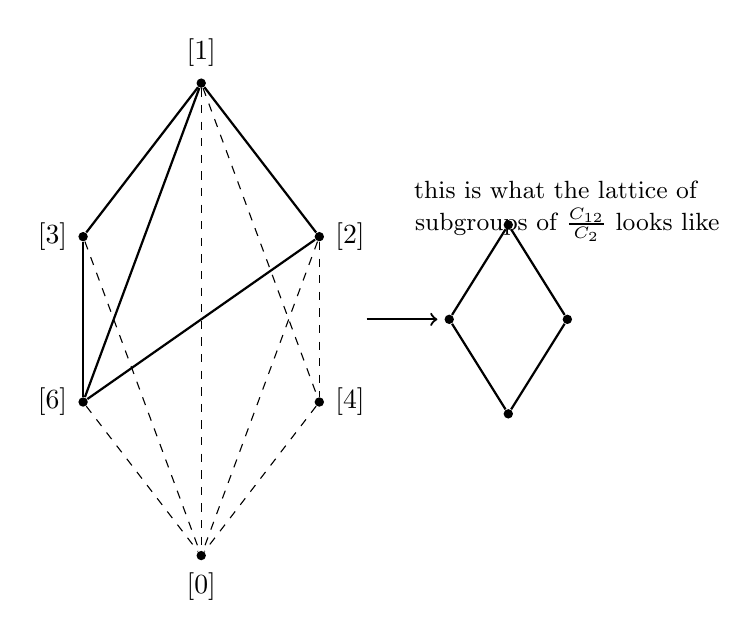
\begin{tikzpicture}[scale=1.5, every node/.style={circle, fill=black, inner sep=1.2pt}]

% Left Lattice Nodes
\node[label=above:{$[1]$}] (n1) at (0,2) {};
\node[label=left:{$[3]$}] (n3) at (-1,0.7) {};
\node[label=right:{$[2]$}] (n2) at (1,0.7) {};
\node[label=left:{$[6]$}] (n6) at (-1,-0.7) {};
\node[label=right:{$[4]$}] (n4) at (1,-0.7) {};
\node[label=below:{$[0]$}] (n0) at (0,-2) {};

% Left Lattice Solid Lines (Subgroups containing [6])
\draw[thick] (n1) -- (n3);
\draw[thick] (n1) -- (n2);
\draw[thick] (n1) -- (n6);
\draw[thick] (n3) -- (n6);
\draw[thick] (n2) -- (n6);

% Left Lattice Dashed Lines (Other subgroups)
\draw[dashed] (n2) -- (n4);
\draw[dashed] (n1) -- (n4);
\draw[dashed] (n1) -- (n0);
\draw[dashed] (n3) -- (n0);
\draw[dashed] (n2) -- (n0);
\draw[dashed] (n6) -- (n0);
\draw[dashed] (n4) -- (n0);

% Transformation Arrow
\draw[->, thick] (1.4,0) -- (2.0,0);

% Right Lattice Nodes
\node (r1) at (2.6,0.8) {};
\node (r2) at (2.1,0) {};
\node (r3) at (3.1,0) {};
\node (r0) at (2.6,-0.8) {};

% Right Lattice Lines
\draw[thick] (r1) -- (r2);
\draw[thick] (r1) -- (r3);
\draw[thick] (r2) -- (r0);
\draw[thick] (r3) -- (r0);

% Handwritten style annotation text
\node[fill=none, draw=none, text=black, align=left, font=\small] at (3.0,1.1) {this is what the lattice of};
\node[fill=none, draw=none, text=black, align=left, font=\small] at (3.1,0.8) { subgroups of $\frac{C_{12}}{C_2}$ looks like};
\node[fill=none, draw=none, text=black, align=left, font=\small] at (3.0,0.5) {};
\node[fill=none, draw=none, text=black, align=left, font=\small] at (3.0,0.3) {};

% Curved Arrow for annotation

\end{tikzpicture}
\end{center}

The result matches the lattice of subgroups of $C_6 \cong C_{12}/C_2$.

\noindent \color{blue} Note: As an exercise show that if $H \subseteq K$ are subgroups of a group $G$ and $H$ is normal in $G$, then $H$ is normal in $K$. \color{black}

\vspace{2em}

\subsection*{Proposition 5.5}
Let $H$ be a normal subgroup of a group $G$. Then for every subgroup $K$ of $G$ containing $H$, $K/H$ may be identified with a subgroup of $G/H$. The function
$$\alpha : \{\text{subgroups } K \text{ of } G \text{ containing } H\} \longrightarrow \{\text{subgroups of } G/H\}$$
defined by $\alpha(K) = K/H$ is a bijection preserving inclusions.

\subsection*{Proof:}
The group $K/H$ consists of the cosets $aH \in G/H$ with $a \in K$, and in this way it is a subset (and obviously a subgroup) of $G/H$. It is also true that if $H \subseteq K \subseteq L$ then $\alpha(K) = K/H \subseteq L/H = \alpha(L)$; and so $\alpha$ preserves inclusions.

Next we verify that $\alpha$ is a bijection and to do this it suffices to write down an inverse function
$$\beta : \{\text{subgroups of } G/H\} \longrightarrow \{\text{subgroups } K \text{ of } G \text{ containing } H\}.$$
Let $K'$ be a subgroup of $G/H$; define $\beta(K')$ to be the subset of $G$:
$$K := \pi^{-1}(K') = \{ a \in G \mid aH \in K' \}.$$

where $\pi : G \longrightarrow G/H$ is the canonical projection. Then $K$ is a subgroup of $G$ and contains $H$ (since $H = \pi^{-1}(e)$ and $e \in K'$).

Next we show that $\alpha$ and $\beta$ are inverses of each other. Indeed
\begin{align*}
\beta(K/H) = \pi^{-1}(K/H) &= \{a \in G \mid \pi(a) \in K/H\} \\
&= \{a \in G \mid aH \in K/H\} \\
&= \{a \in G \mid a \in K\} = K.
\end{align*}
So $(\beta \circ \alpha)(K) = K$. On the other hand taking $\beta(K') = K$,
$$\alpha(K) = K/H = \pi(K) = \pi(\pi^{-1}(K')) = K'.$$
Thus $(\alpha \circ \beta)(K') = K'$.

\vspace{2em}

\noindent The correspondence preserves normal subgroups. The following statement is usually known as the \color{red}third isomorphism theorem\color{black}:
\subsection*{\color{blue}Proposition 5.6}
Let $H$ be a normal subgroup of $G$, and let $N$ be a subgroup of $G$ containing $H$. Then $N/H$ is normal in $G/H$ if and only if $N$ is normal in $G$, and in this case
$$\frac{G/H}{N/H} \cong \frac{G}{N}$$

\color{black}
\subsection*{Proof}
If $N$ is normal, then consider the projection
$$G \longrightarrow \frac{G}{N}:$$
the subgroup $H$ is contained in $N$, which is the kernel of this homomorphism, so we obtain by Theorem 4.12 an induced homomorphism
\vspace{8em}

\begin{tikzpicture}[remember picture, overlay]
\node[draw=black, fill=white, text=black, align=left, font=\footnotesize, thick] at (5.3, 2.3) {
    $\ker\mu = \{gH \in G/H \mid \mu(gH) = N\}$ \\
    $\phantom{\ker\mu} = \{gH \in G/H \mid gN = N\}$ \\
    $\phantom{\ker\mu} = \{gH \in G/H \mid g \in N\} = N/H$
};
\end{tikzpicture}

\[
\begin{tikzcd}
G \arrow[rd, "\pi_H"'] \arrow[rr, "\pi_N", blue] &  & G/N \\
 & G/H \arrow[ru, "\mu"'] &
\end{tikzcd}
\]
\noindent The subgroup $N/H$ of $G/H$ is the kernel of this homomorphism; therefore it is normal.

Conversely, if $N/H$ is normal in $G/H$, consider the composition
\[
\begin{tikzcd}
G \arrow[r, "\pi", two heads] & G/H \arrow[r, "\widetilde{\pi}", two heads] & \frac{G/H}{N/H}
\end{tikzcd}
\]
The kernel of this homomorphism
\begin{align*}
\ker(\widetilde{\pi} \circ \pi) &= \{ g \in G \mid (\widetilde{\pi} \circ \pi)(g) = N/H \} \\
&= \{ g \in G \mid \widetilde{\pi}(gH) = N/H \} \\
&= \{ g \in G \mid gH \in N/H \}
\end{align*}


\[
= \{g \in G \mid g \in N\} = N.
\]
Furthermore, this homomorphism is surjective; hence the stated isomorphism
\[
\frac{G/H}{N/H} \cong G/N \qquad \text{follows from Corollary 5.2.}
\]

\vspace{1em}

\subsection*{\underline{\large $HK/H$ \text{ and } $K/(H \cap K)$}}

In the previous section, we dealt with two `nested' subgroups $H \subseteq K$ of a group $G$. We will now consider the case when two subgroups $H$ and $K$ are not nested.

If $H$ and $K$ are two subgroups of a group $G$, then
\[
HK = \{hk \mid h \in H, \, k \in K\}
\]
is a subset. Whenever \underline{$G$ is commutative}, then $HK$ is a subgroup of $G$. Another instance where $HK$ is a subgroup is when one of the subgroups is normal. The following is usually called the second isomorphism theorem.

\vspace{1em}

\subsection*{\underline{Proposition 5.7}}
Let $H$ and $K$ be subgroups of a group $G$, and assume that $H$ is normal in $G$. Then
\begin{enumerate}
    \item $HK$ is a subgroup of $G$, and $H$ is normal in $HK$;
    \item $H \cap K$ is normal in $K$, and  \[
    \frac{HK}{H} \cong \frac{K}{H \cap K}
    \]
\end{enumerate}


\subsection*{\underline{Proof:}}
To verify that $HK$ is a subgroup of $G$ when $H$ is normal, note that $HK$ is the union of all cosets $Hk$, with $k \in K$; that is,


\[
HK = \pi^{-1}(\pi(K)),
\]
where $\pi : G \longrightarrow G/H$ is the canonical projection. Since $\pi(K)$ is a subgroup of $G/H$, $HK$ is a subgroup. Since $H$ is normal in $G$ and $H$ is a subgroup of $HK$, we have $H$ normal in $HK$.

\vspace{1em}

For the second part, consider the homomorphism
\[
\varphi : K \longrightarrow HK/H
\]
sending $k \in K$ to the coset $Hk$ (that is, the inclusion $K \lhook\joinrel\longrightarrow HK$ followed by the canonical projection to the quotient, i.e. $K \lhook\joinrel\longrightarrow HK \longrightarrow HK/H$).


This is surjective; indeed, every element of $HK/H$ may be written as a coset
\[
Hhk, \quad h \in H, \, k \in K;
\]
but $Hhk = Hk$ and so $Hhk = \varphi(k)$ is in the image of $\varphi$. By corollary 5.2
\[
\frac{HK}{H} \cong \frac{K}{\ker \varphi}
\]

\vspace{1em}

\noindent \underbar{What is $\ker \varphi$?}
\begin{align*}
\ker \varphi = \{k \in K \mid \varphi(k) = e\} &= \{k \in K \mid Hk = H\} \\
&= \{k \in K \mid k \in H\} \\
&= H \cap K.
\end{align*}
Thus we have the required results.

\vspace{2em}

\subsection*{\underline{The index and Lagrange's theorem}}
The notation $G/H$ is used to denote the set of left cosets of $H$. So $G/H$ is in general a set, and it is a group when $H$ is a normal subgroup of $G$.



\subsection*{\underline{Definition 5.8}}
The index of $H$ in $G$, denoted $[G:H]$, is the number of elements $|G/H|$ of $G/H$, when this is finite and $\infty$ otherwise.

\vspace{1em}

\noindent So, $[G:H]$ (if finite) refers to the number of distinct left-cosets of $H$ in $G$, regardless of whether $H$ is normal in $G$.

\vspace{2em}

\subsection*{\underline{Lemma 5.9}}
Let $H$ be a subgroup of a group $G$. Then $\forall g \in G$ the functions
\begin{align*}
H \longrightarrow gH, \quad h \mapsto gh \\
H \longrightarrow Hg, \quad h \mapsto hg
\end{align*}
are bijections.



\subsection*{\underline{Proof}}
Both functions are surjective by definition of coset. Cancellation implies that they are injective.

\vspace{1.5em}

\subsection*{\underline{Corollary 5.10} (Lagrange's theorem)}
If $G$ is a finite group and $H \subseteq G$ is a subgroup, then $|G| = [G:H] \cdot |H|$. In particular, $|H|$ is a divisor of $|G|$.

\vspace{1.5em}

\subsection*{\underline{Proof}}
Indeed, $G$ is the disjoint union of $|G/H|$ distinct cosets $gH$, and $|gH| = |H|$ by Lemma 5.9.

Thus
\begin{align*}
|G| &= [G:H] \cdot |gH| \\
|G| &= [G:H] \cdot |H|
\end{align*}

\vspace{1.5em}

\subsection*{\underline{Example 5.11}}
The order $|g|$ of any element $g$ of a finite group $G$ is a divisor of $|G|$; indeed, $|g|$ equals the order of the subgroup $\langle g \rangle$ generated by $g$.

\vspace{2em}

\noindent \underbar{Note}: Thus, $g^{|G|} = e_G$ for all finite groups $G$, for all $g \in G$.

\subsection*{\underline{Example 5.12}}
If $|G|$ is a prime integer $p$, then necessarily $G \cong \mathbb{Z}_p$.

Indeed, let $g \in G$ be any non-identity element; then $\langle g \rangle$ is a subgroup of $G$, of order $>1$. By Lagrange's theorem $|\langle g \rangle| = p = |G|$; that is, $G \cong \langle g \rangle$ is cyclic of order $p$, as claimed.

\vspace{1.5em}

\subsection*{\underline{Example 5.13} (Fermat's little theorem)}
Let $p$ be a prime integer, and let $a$ be any integer. Then $a^p \equiv a \pmod p$.

Indeed, this is clear if $a$ is a multiple of $p$; if $a$ is not a multiple of $p$, then the class $[a]_p$ modulo $p$ is non-zero, so it is an element of the group $(\mathbb{Z}_p)^*$, which has order $p-1$. Thus
\[
[a]_p^{p-1} = [1]_p;
\]
hence $[a]_p^p = [a]_p$ as desired.

\vspace{2em}

The index is a well-behaved invariant. It is clearly multiplicative, in the sense that if $H \subseteq K$ are subgroups of $G$, then
\[
[G:H] = [G:K] \cdot [K:H],
\]
provided that these numbers are finite. In addition, if $H$ and $K$ are subgroups of $G$ and $H$ is normal, then
\[
|HK| = \frac{|H| \cdot |K|}{|H \cap K|}
\]
(again if the orders are finite), this follows immediately from isomorphism in preposition 5.
\subsection*{\underline{Revisit Homomorphisms}}
Let $\varphi : G \to G$ be a homomorphism of groups. Then $\varphi$ is said to be an epimorphism if and only if $\varphi$ is surjective

\subsection*{\underline{Group Actions}}
Let $G$ be a group and let $A$ be a set and $\text{Hom}_{\text{set}}(A,A)$ be the set of functions from $A$ to $A$.

\subsection*{\underline{Definition 6.1}}
An action of a group $G$ on a set $A$ is a set-function
\[
\rho : G \times A \longrightarrow A
\]
such that $\rho(e_G, a) = a$ for all $a \in A$ and $(\forall g, h \in G), (\forall a \in A)$
\[
\rho(gh, a) = \rho(g, \rho(h, a)).
\]

\vspace{1em}

\noindent Indeed, given a function $\rho$ satisfying these conditions, we can define
\[
\sigma : G \longrightarrow \text{Hom}_{\text{set}}(A,A)
\]
by $\sigma(g)(a) = \rho(g, a)$. \\
(This defines $\sigma(g)$ as a set function $A \rightarrow A$, as needed.)

This function preserves the operation, because

\begin{align*}
\sigma(gh)(a) = \rho(gh, a) = \rho(g, \rho(h, a))
&= \sigma(g)(\rho(h,a)) = \sigma(g)(\sigma(h)(a)) \\
&= \sigma(g) \circ \sigma(h)(a).
\end{align*}


Particularly, this verifies that $\sigma(g^{-1})$ acts as the inverse of $\sigma(g)$; because $(\forall a \in A)$,
\begin{align*}
\sigma(g^{-1}) \circ \sigma(g)(a) &= \sigma(g^{-1}g)(a) \\
&= \sigma(e_G)(a) \\
&= \rho(e_G, a) = a.
\end{align*}

\vspace{1em}

\noindent So we see that the image of $\sigma$ consists of invertible set-functions; $\sigma$ is acting as a function
\[
\sigma : G \longrightarrow S_A
\]
and we have verified above that it is a homomorphism as required.

Conversely, given a homomorphism $\sigma : G \longrightarrow S_A$, define $\rho : G \times A \longrightarrow A$ by $\rho(g,a) = \sigma(g)(a)$. Then
\begin{align*}
\rho(e_G, a) &= \sigma(e_G)(a) \\
&= \text{id}(a)
\end{align*}
where $\sigma(e_G)$ is the identity permutation.

\vspace{2em}

\noindent Next, for all $g_1, g_2 \in G$ and $a \in A$,
\begin{align*}
\rho(g_1 g_2, a) &= \sigma(g_1 g_2)(a) \\
&= \sigma(g_1) \circ \sigma(g_2)(a) \\
&= \sigma(g_1)(\sigma(g_2)(a)) \\
&= \rho(g_1, \rho(g_2, a)).
\end{align*}


Thus we have shown that $\rho$ is an action of $G$ on $A$.

From what follows we will write $\rho(g,a)$ as $g \cdot a$ so that the above will read as follows
\[
\boxed{
\begin{aligned}
e_G \cdot a &= a \quad \text{and} \\
(g_1 g_2) \cdot a &= g_1 \cdot (g_2 \cdot a)
\end{aligned}
}
\]

\vspace{1em}

\subsection*{\underline{Note:}}
If $G$ acts on $A$, then $e_G \cdot a = a$ for every $a \in A$; the action of a group $G$ on a set $A$ is \underline{faithful} if and only if the identity $e_G$ is the only element $g \in G$ such that $g \cdot a = a$ for all $a \in A$, that is, fixing every element of $A$.

An action is \underline{\smash{\textcolor{blue}{free}}} if the identity $e_G$ is \underline{the only element} fixing \underline{any} element of $A$.

\vspace{1em}

\noindent {\color{red} $\bullet$ Include another definition on the next page.}

\subsection*{\underline{Example 6.2}}
{\color{blue}$\bullet$} Every group $G$ acts in a natural way on the underlying set $G$. The function $\rho : G \times G \longrightarrow G$ is simply the group operation:

\[
(\forall g, a \in G) : \rho(g, a) = ga.
\]
This is referred to as the action by left multiplication of $G$ on itself.

{\color{blue}$\bullet$} There is another natural way to act with $G$ on itself, by conjugation: define $\rho : G \times G \longrightarrow G$ by
\[
\rho(g, h) = ghg^{-1}.
\]
This is indeed an action: $\forall g, h, k \in G$,
\[
\rho(g, \rho(h, k)) = g\rho(h, k)g^{-1} = g(hkh^{-1})g^{-1}
\]

\vspace{5em}

\subsection*{\underline{Definition}}
An action of a group $G$ on a set $A$ is faithful (or effective) if the corresponding group homomorphism
\[
\rho : G \longrightarrow S_A
\]
is injective.


\subsection*{\underline{Example 6.3}}
Consider the set $G/H$ of left-cosets of any subgroup $H$ of a group $G$. The group $G$ acts on the set $G/H$ as follows:
\begin{align*}
G \times G/H &\longrightarrow G/H \\
(g, \, aH) &\longmapsto (ga)H
\end{align*}

\vspace{1em}

\subsection*{\underline{Theorem 6.4} (Cayley's theorem)}
Every group acts faithfully \underline{on some set}. That is, every group may be realized as a subgroup of a permutation group.

\vspace{1em}

\subsection*{\underline{Proof}}
Indeed, observe that the left multiplication action of $G$ on itself is faithful.

\vspace{1.5em}

\noindent {\color{blue}Note: A set, $A$, carrying an action of a group $G$ on it is referred to as a $G$-set.}

\vspace{3em}

So far what we discussed are left actions of a group $G$ on some set $A$. One can also talk about right actions where in this case we have a map say
\begin{align*}
\rho : A \times G &\longrightarrow A \\
(a, g) &\longmapsto a \cdot g
\end{align*}


However note that every right action may be turned into a left action: From now on, we mean left action whenever we say action.

\vspace{1em}

\subsection*{\underline{Transitive actions}}

\subsection*{\underline{Definition 6.5}}
An action of a group $G$ on a (nonempty) set $A$ is transitive if $\forall a, b \in A$, $\exists g \in G$ such that $b = ga$.

\vspace{1em}

For example, the left multiplication action of a group on itself is transitive.

\vspace{1em}

\subsection*{\underline{Definition 6.6}}
The orbit of $a \in A$ under an action of a group $G$ is the set

\vspace{3em}

\[
\mathcal{O}_G(a) := \{ga \mid g \in G\}.
\]

\vspace{1em}

\subsection*{\underline{Definition 6.7}}
Let $G$ act on a set $A$, and let $a \in A$. The stabilizer subgroup of \underline{$a$} consists of the elements of $G$ which fix \underline{$a$} :
\[
\text{Stab}_G(a) := \{g \in G \mid ga = a\}
\]



Orbits of an action of a group $G$ on a set $A$ form a partition of $A$; and we have an induced, transitive action of $G$ on each orbit. So in a sense we can understand all actions if we understand transitive actions.


\vspace{1em}

\subsection*{\underline{\color{blue}Proposition 6.8}}
{\color{blue}
Let $G$ be a group and $X$ be a $G$-set. Then for each $x \in X$,
\[
|\mathcal{O}_G(x)| = [G : \text{Stab}_G(x)].
\]
}

\vspace{3em}

\subsection*{\underline{Proof}}
We first need to show that there exists a bijective map between $\mathcal{O}_G(x)$ and $G/\text{Stab}_G(x)$. Let $\theta : \mathcal{O}_G(x) \longrightarrow G/\text{Stab}_G(x)$ be a map defined by $\theta(g \cdot x) = g \, \text{Stab}_G(x)$. Next we will show that $\theta$ is well defined: let $g_1 \cdot x = g_2 \cdot x$, then $g_2^{-1} g_1 \cdot x = x$. This means that $g_2^{-1} g_1 \in \text{Stab}_G(x)$ and this implies that $g_1 \, \text{Stab}_G(x) = g_2 \, \text{Stab}_G(x)$. So $\theta$ is well defined.

Next we show that $\theta$ is injective; let $\theta(g_1 \cdot x) = \theta(g_2 \cdot x)$, then $g_1 \, \text{Stab}_G(x) = g_2 \, \text{Stab}_G(x)$ which implies that $g_2^{-1} g_1 \in \text{Stab}_G(x)$ and so $g_2^{-1} g_1 \cdot x = x$ and so $g_1 \cdot x = g_2 \cdot x$. Thus $\theta$ is injective. Now $\theta$ is surjective because for any $g \, \text{Stab}_G(x) \in G/\text{Stab}_G(x)$
there exists $g \cdot x \in \mathcal{O}_G(x)$ such that $g \, \text{Stab}_G(x) = \theta(g \cdot x)$. So we have a bijection of sets and so these sets must have the same cardinality. This is the cardinality of the orbit of $x$ is equal to the number of left cosets of $\text{Stab}_G(x)$ in $G$ which is equal to the index of $\text{Stab}_G(x)$ in $G$.

\vspace{2em}

Assume $G$ acts on a set $A$. Let $Z$ be the set of fixed points of the action, i.e.
\[
Z = \{a \in A \mid (\forall g \in G) : ga = a\}.
\]
Note that $a \in Z$ if and only if $\text{Stab}_G(a) = G$. That the orbit of \underline{$a$} has length \underline{one} ({\color{blue}$\mathcal{O}_G(a) = \{a\}$}).

\vspace{1.5em}

\subsection*{\underline{\color{blue}Proposition 6.9}}
Let $A$ be a finite set, and let $G$ be a group acting on $A$. Then
\[
|A| = |Z| + \sum [G : \text{Stab}_G(a)].
\]

\vspace{1em}

\subsection*{\underline{Proof}}
The orbits form a partition of $A$, and $Z$ contains orbits all of length one, hence
\[
|A| = |Z| + \sum_{a \in S} |\mathcal{O}_G(a)|
\]

where $\mathcal{O}_G(a)$ denotes the orbit of $a$ which have length $>1$; but $|\mathcal{O}_G(a)| = [G : \text{Stab}_G(a)]$ by Proposition 6.8.

\vspace{1.5em}

\subsection*{\underline{Center, Centralizer and Conjugacy classes}}
Recall the action of $G$ on itself by conjugation; that is,

\vspace{3em}

\[
\rho : G \times G \longrightarrow G \quad \text{with} \quad \rho(g,a) = gag^{-1}.
\]
We know that this action induces a certain group homomorphism
\[
\sigma : G \longrightarrow S_G
\]
from $G$ to the permutation group on $G$. Pertaining to this action we observe the following:

\vspace{1.5em}

\subsection*{\underline{Definition 6.10}}
The center of $G$, denoted $Z(G)$, is the subgroup $\ker \sigma$ of $G$.

Concretely, the center of $G$ is
\[
Z(G) = \{g \in G \mid (\forall a \in G) : ga = ag\}
\]
Indeed, $\sigma(g)$ is the identity in $S_G$ if and only if $\sigma(g)$ acts as the identity on $G$; that is, if and only if $gag^{-1} = a$ for all $a \in G$; that is, if and only if $g$ commutes with all elements of $G$. In other words, the center is the set of fixed points in $G$ under the conjugation action.


\noindent Note that the center of a group $G$ is normal.

\vspace{2em}

{\color{blue}
A group $G$ is commutative if and only if $Z(G) = G$, that is, if and only if the conjugation action is trivial on $G$.
}

\vspace{1.5em}

\subsection*{\underline{\color{blue}Lemma 6.11}}
{\color{blue}
Let $G$ be a finite group, and assume $G/Z(G)$ is cyclic. Then $G$ is commutative (and hence $G/Z(G)$ is trivial).
}

\vspace{1.5em}

\subsection*{\underline{Proof}}

As $G/Z(G)$ is cyclic, there exists an element $g \in G$ such that the class $gZ(G)$ generates $G/Z(G)$. Then $\forall a \in G$,
\[
aZ(G) = (gZ(G))^r
\]
for some $r \in \mathbb{Z}$; that is, there is an element $z \in Z(G)$ of the center such that
\[
a = g^r z
\]
(this is because $a$ and $g^r$ are in the same equivalence class).

If now $a, b$ are in $G$, then $aZ(G)$ and $bZ(G)$ are in $G/Z(G)$ and so


\[
a = g^r z \quad \text{and} \quad b = g^s w
\]
for some $s \in \mathbb{Z}$ and $w \in Z(G)$; \\
(by the same argument that $gZ(G)$ generates $G/Z(G)$) \\
but
\[
ab = (g^r z)(g^s w) = g^{r+s} zw = (g^s w)(g^r z) = ba
\]
(Note that in the above the fact that $z$ and $w$ commute with every element of $G$ was used).

As $a$ and $b$ are arbitrary, this shows that $G$ is commutative.

\vspace{1.5em}

We now consider the stabilizer of $a \in G$ under conjugation:

\vspace{1.5em}

\subsection*{\underline{Definition 6.12}}
The Centralizer (or normalizer) $Z_G(a)$ of $a \in G$ is its stabilizer under conjugation.

Thus
\[
Z_G(a) = \{g \in G \mid gag^{-1} = a\} = \{g \in G \mid ga = ag\}
\]
consists of those elements in $G$ which commute with \underline{$a$}.

\vspace{2em}

In particular, $Z(G) \subseteq Z_G(a)$ for all $a \in G$; in fact $Z(G) = \bigcap_{a \in G} Z_G(a)$. Obviously,
\[
a \in Z(G) \iff Z_G(a) = G.
\]


\subsection*{\underline{Definition 6.13}}
The conjugacy class of $a \in G$ is the orbit $\mathcal{O}_G(a)$ of $a$ under the conjugation action. Two elements $a, b$ of $G$ are conjugate if they belong to the same conjugacy class.

\vspace{1.5em}

\subsection*{\underline{The Class Formula}}

\subsection*{\underline{Proposition 6.14} (Class formula)}
Let $G$ be a finite group. Then
\[
|G| = |Z(G)| + \sum_{a \in A} [G : Z_G(a)]
\]
where $A \subseteq G$ is a set containing one representative for each conjugacy class in $G$ containing more than one element.

\vspace{3em}

\subsection*{\underline{Proof}}
The set of fixed points is $Z(G)$, and the stabilizer of \underline{$a$} is the centralizer $Z_G(a)$; apply Proposition 6.9.


The class equation is very useful. In applying it, keep in mind that every summand on the right (that is, both $|Z(G)|$ and each $[G : Z_G(a)]$) is a divisor of $|G|$; this fact alone often suffices to draw conclusions about $G$.

\vspace{1.5em}

\subsection*{\underline{Example 6.15}}
Consider a group $G$ of order $6$; what are the possibilities of its class formula?

If $G$ is commutative, then the class formula will tell us very little:
\[
6 = 6.
\]
If $G$ is not commutative, then its center must be trivial. The other summands, which are the non-trivial conjugacy classes, have sizes greater than $1$ and must divide $6$; that is, there are no choices:
\[
6 = 1 + 2 + 3
\]
is the only option.
